\documentclass{article}
\usepackage[utf8]{inputenc}
\usepackage[brazil]{babel}
\usepackage{epsfig}
\usepackage{fancyhdr}
\usepackage{indentfirst} %In­dent first para­graph af­ter sec­tion header
\usepackage{titlesec}
\usepackage{amsmath}
\usepackage{amsthm}

\pagestyle{empty}

\headheight 40mm      %
\oddsidemargin 2.0mm  %
\evensidemargin 2.0mm %
\topmargin -40mm      %
\textheight 250mm     %
\textwidth 160mm      %
%
\newcounter{execs}
\setcounter{execs}{0}
\newcommand{\exec}[0]{\addtocounter{execs}{1}\item[\textbf{\arabic{execs}.}]}

\fancypagestyle{first}
{
\pagestyle{fancy}
}
%%%%%%%%%%%%%%%%%%%%%%%%%%%%%%%%%%%%%%%%%%%%%%%%%%%%%%%%
%%%%%%%%%%%%%%%%%%%%%%%%%%%%%%%%%%%%%%%%%%%%%%%%%%%%%%%%
% PLEASE, EDIT THIS!
\fancyhead[LO]{\small $6^a$ Lista \\ 
                DCC008 - Cálculo Numérico  \\
                \textbf{Entrega: 28 de Novembro de 2018} }

\fancyhead[RO]{\small Universidade Federal de Juiz de Fora - UFJF \\ 
                Departamento de Ciência da Computação \\
               \textit{Nome: Thiago de Almeida}\\
               \textit{Nome: Renan Nunes}}


\begin{document}
\thispagestyle{first}
%    \noindent \textbf{Obs1.:}  Escolha um ou mais métodos de interpolação dado em aula para resolver os problemas abaixo.
%    
%    \noindent \textbf{Obs2.:}  Discuta os resultados.

\begin{itemize}

\exec Seja a função:
\begin{equation}\label{solexat1}
u(x) = c_1 e^{-\tfrac{x}{\sqrt{\varepsilon}}} + c_2 e^{\tfrac{x}{\sqrt{\varepsilon}}}+1
\end{equation}
com $c_1 = -1-c_2$ e $c_2 = \dfrac{e^{-\tfrac{1}{\sqrt{\varepsilon}}}-1}
{e^{\tfrac{1}{\sqrt{\varepsilon}}}-e^{-\tfrac{1}{\sqrt{\varepsilon}}}}$.
Adotando $x\in [0,1]$ e $\varepsilon=0.001$, faça:

\begin{itemize}

\item[a)] Ajuste a função $u(x)$ por mínimos quadrados utilizandpo diferentes ordens ($n=1,2,3,4,5$) e apresente gráficos comparando com a solução exata \eqref{solexat1}. Para isso, utilize a quadratura de Gauss para integração numérica utilizando $n+1$ pontos. 

\item [b)] Repita o item (a) dividindo o intervalo $[0,1]$ em 25 subintervalos iguais e utilize ordem $n=1$ em cada subintervalo. 

\item [c)] Calcule o erro de todas as curvas ajustadas nos itens (a) e (b) utilizando a norma L2, que pode ser definida como:
$$
\|u(x)-u_h(x)\|_0 =\sqrt{ \sum_{i=0}^{K-1} \int_{x_i}^{x_{i+1}} (u(x)-u_h(x))^2~dx}
$$
onde $u_h(x)$ é a curva ajustada por mínimos quadrados e $K$ é o número de partições do domínio (neste caso, $x_0=0$ e $x_K=1$). Aplique a regra $3/8$ de simpson para o cálculo da integral. Construa uma tabela com os resultados.

\end{itemize}


\newpage
\text Para a resolução da função acima foram usandos os métodos de integração de Newton Contes e o método da Quadratura de Gauss, além do método dos Mínimos Quadrados e da norma L2.

\begin{itemize}

\item[a)] Ajustando a função por mínimos quadrados e utilizando a Quadratura de Gauss, é possível obter os seguintes resultados.

\begin{figure}[!htb]
\centering
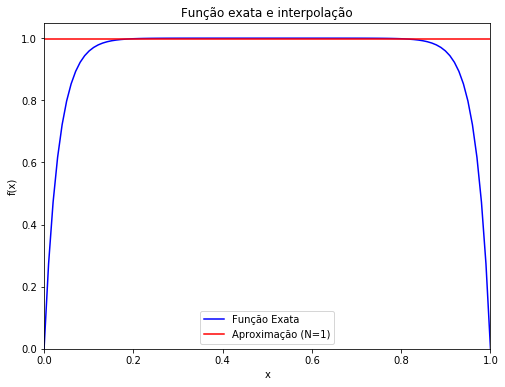
\includegraphics [width=7cm,height=7cm]{LetraA/Ordem1.png}
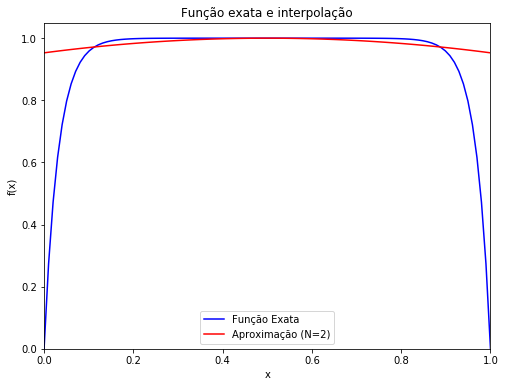
\includegraphics [width=7cm,height=7cm]{LetraA/Ordem2.png}
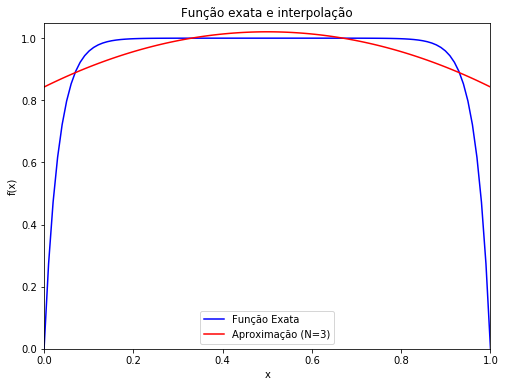
\includegraphics [width=7cm,height=7cm]{LetraA/Ordem3.png}
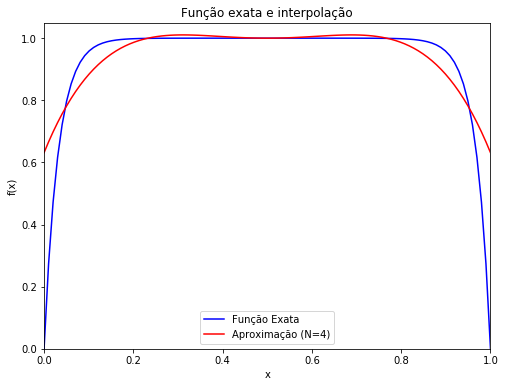
\includegraphics [width=7cm,height=7cm]{LetraA/Ordem4.png}
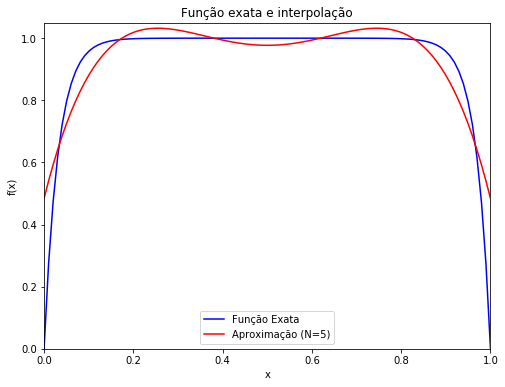
\includegraphics [width=7cm,height=7cm]{LetraA/Ordem5.png}
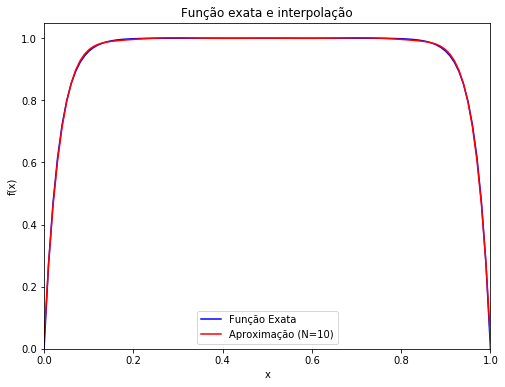
\includegraphics [width=7cm,height=7cm]{LetraA/Ordem10_Extra.png}
\end{figure}

\item[-] O método de Integração funciona bem para uma maior quantidade de pontos, melhorando seu ajuste conforme o n aumenta e se estabilizando em n = 10.

\newpage

\item[b)] Dividindo o intervalo em 25 subintervalos e com ordem N = 1 para cada intervalo obtem-se:

\begin{figure}[!htb]
\centering
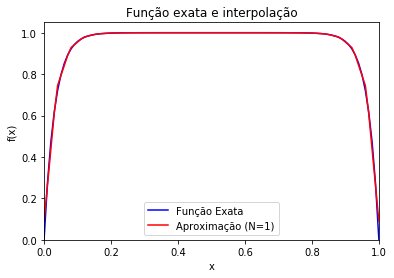
\includegraphics [width=10cm,height=10cm]{LetraB/N1.png}
\end{figure}

\item[c)] Utilizando o erro do calculo da norma L2, com aplicação da regra de Simpson 3/8, obtem-se a seguinte tabela:

\begin{table}[h]
\centering
  \begin{tabular}{|l|l|l|ll}
   $N$ & $Erro$ $da$ $Norma$ $L2$ $Letra$ $A$ & $Erro$ $da$ $Norma$ $L2$ $Letra$ $B$ \\
    \hline
    1 &   0.1773886390985522 & 0.0161685851792788 \\
    2 &   0.16372271194605556 & ----------------- \\
    3 &   0.13677813068526803 & ----------------- \\
    4 &   0.09349994506603918 & ----------------- \\
    5 &   0.07132167453594482 & ----------------- \\
    \hline
  \end{tabular}
  \caption{Resultado dos Erros da Norma L2}
\end{table}

\item[-] Após a implementação e a observação do comportamento dos métodos, pode-se concluir que o número de pontos e partições influência profundamente no resultado do método, deixando-o mais próximo da solução exata.

\end{itemize}

\end{itemize}

\end{document}
